\chapter{Kravspecifikation (SK)}

Der er blevet lavet en kravspecifikation, som tager udgangspunkt i usecase diagrammet på figur \ref{lab:usecasediagram}. Usecase diagrammet viser hvilke usecases som Bruger og Golfbane har kontakt til, den komplette usecase beskrivelse kan ses i projektdokumentationen i kapitel 2, Kravspecifikation. 

%% !!! Usecase diagram !!!
\begin{figure}[H] \centering
\vspace*{\fill}
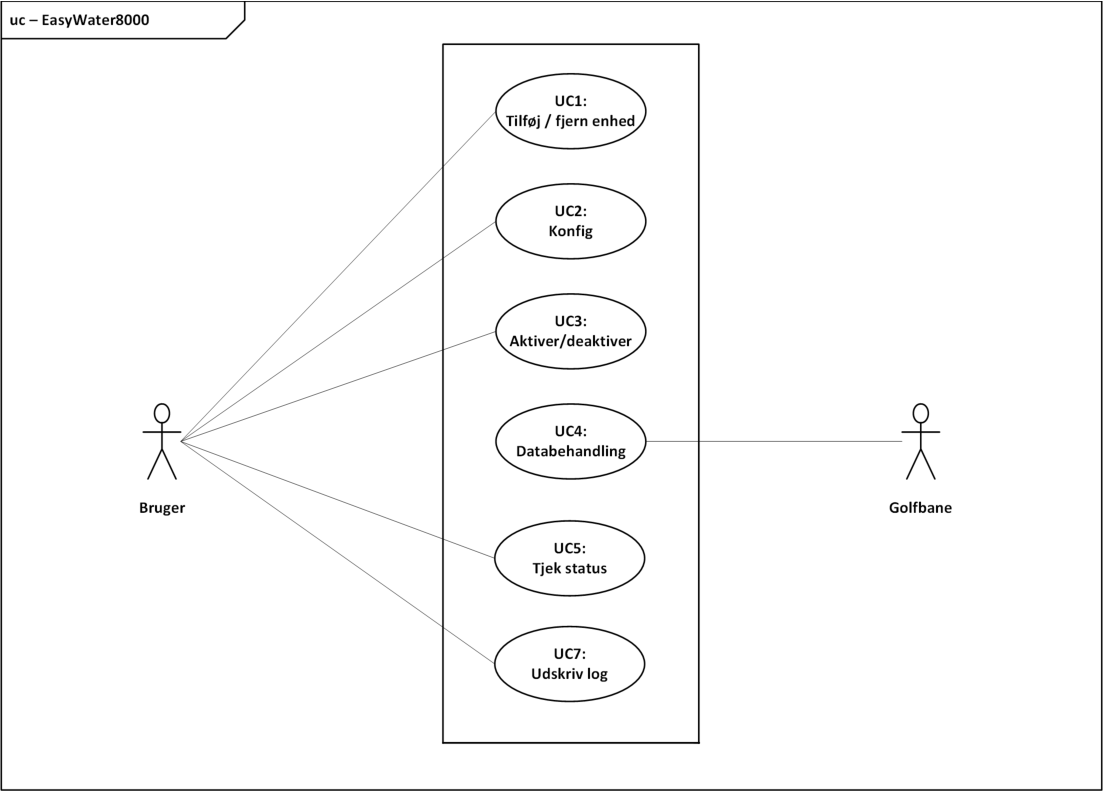
\includegraphics[width=\textwidth]{Billeder/Usecase_Diagram}
\caption{Usecase diagram}
\label{lab:usecasediagram}
\vspace*{\fill}
\end{figure}

Herunder ses en beskrivelse af aktørerne i EasyWater8000.

\begin{table}[!htbp] \centering
	\begin{tabular}{|p{2.5cm}|p{11.5cm}|}
	\hline
		\textbf{Aktør navn} & \textbf{Beskrivelse} \\\hline
		Bruger & Bruger vil normalt være greenkeeperen. Det er vedkommende som kontrollerer og betjener systemet. (Primær) \\\hline

		Golfbane & De almene omgivelser på golfbanen, som har indflydelse på systemets sensorer. Det indebærer temperatur, fugtighed og bevægelse i området omkring systemet. (Sekundær) \\\hline
	\end{tabular}
\end{table}

\subsection{Ikke-funktionelle krav}
Herunder ses en beskrivelse af de ikke-funktionelle krav i EasyWater8000.
% Ikke-funktionelle krav
\begin{enumerate}

\subsubsection*{Brugbarhed}
\item Opsætningen skal ske af autoriseret personale
\item GUI skal kunne benyttes af bruger efter gennemlæst manual


\subsubsection*{Pålidelighed}
\item Software IDLE tid: minimum 1 måned uden restart


\subsubsection*{Ydeevne}
\item Master skal kunne håndtere op til 18 enheder
\item Sprinkler skal kunne vande et areal af 360$^{\circ}$ med radius på 3.5 m 
\item Der skal kunne tilføjes yderligere Enheder efter opsætning af systemet
\item Master skal hente data fra tilkoblede Enheder hvert 15. minut
\item Enhed skal hente data fra sensorer i et fast interval


\subsubsection*{Vedligeholdelse}
\item Enheder skal være udskiftelige uden at det er nødvendigt at tilgå sensorer eller sprinkler
\item Sprinklere skal være let tilgængelige for personale


\subsubsection*{Enheder}
\item Enhed skal kunne operere autonomt efter denne er sat op fra Master
\item Enheder skal gemme log-information ifm. vanding og målinger, indtil Master udlæser denne

\end{enumerate}

\subsubsection*{Begrænsninger}
\begin{itemize}
\item Der udarbejdes en skaleret prototype, da vi ikke har adgang til en hel golfbane
\item Grundet tidsbegrænsninger udvikles der ikke et fuldt system 
\item Som minimum skal der produceres en funktionel Master og én komplet Enhed
\item Systemet udvikles således, at der til hver sprinkler tilhører en pumpe. Denne løsning vil ikke vælges i en produktionsudgave, her vil der være én vandforsyning, med et tryk stort nok, til at tilføre samtlige sprinklere den nødvendige mængde vand.
% Skal uddybes i fremtidigt atbejde ?
\end{itemize}



